\chapter{Ottimizzazione Matematica: Script 8 (Markowitz Pura)}

Se la simulazione stocastica (Script 7) si limita a proiettare gli scenari futuri in base ai pesi decisi empiricamente dall'utente, l'ottimizzazione Media-Varianza, implementata analiticamente nello script R \texttt{previsione\_8\_markowitz\_pura.R}, ha un obiettivo inverso: ricercare iterativamente nello spazio N-dimensionale il vettore dei pesi $\vec{w}$ che massimizzi matematicamente il rapporto rischio-rendimento.

\section{Modello Media-Varianza e Frontiera Efficiente}
Dato un portafoglio composto da $N$ asset, e definito $\vec{w} = [w_1, w_2, \dots, w_N]^T$ il vettore dei pesi (soggetto al vincolo convesso $\sum_{i=1}^{N} w_i = 1$), il rendimento atteso del portafoglio \`e un'operazione lineare:
\begin{equation}
E[R_p] = \vec{w}^T \vec{\mu}
\end{equation}
dove $\vec{\mu}$ \`e il vettore colonna dei rendimenti attesi. La \emph{varianza} del portafoglio (il "rischio" del capitale), essendo influenzata dalle correlazioni inter-asset, \`e calcolata in forma quadratica:
\begin{equation}
\sigma_p^2 = \vec{w}^T \Sigma \vec{w}
\end{equation}

Lo Script 8 genera casualmente 20.000 vettori di pesi $\vec{w}$ esplorando esaustivamente l'iper-spazio dei portafogli ammissibili, proiettandoli in un grafico 2D ($\sigma_p$ sulle ascisse, $E[R_p]$ sulle ordinate). Il margine superiore sinistro della "nuvola" generata \`e la celebre \textbf{Frontiera Efficiente}.

\section{Identificazione del Punto Ottimo (Tangency Portfolio)}
L'obiettivo algoritmico dello Script 8 non \`e trovare il rendimento assoluto pi\`u alto (che coinciderebbe banalmente con un peso 100\% sull'asset pi\`u volatile), ma trovare il \emph{Tangency Portfolio}, ovvero il punto in cui la pendenza della \emph{Capital Allocation Line} (CAL) \`e massima. Questo si ottiene massimizzando l'\textbf{Indice di Sharpe}:
\begin{equation}
\max_{\vec{w}} \left( \text{Sharpe Ratio} \right) = \max_{\vec{w}} \left( \frac{\vec{w}^T \vec{\mu} - R_f}{\sqrt{\vec{w}^T \Sigma \vec{w}}} \right)
\end{equation}
dove $R_f$ \`e il \emph{risk-free rate} (impostato matematicamente al 3.0\% annuo nel nostro codice).

\section{Analisi Comparativa: Scarto di Efficienza}
L'esecuzione dello Script 8 dimostra matematicamente l'inefficienza di allocazioni empiriche. Confrontando il portafoglio "utente" (es. 60/20/20 su VWCE, Oro, Petrolio) con il vettore ottimo $\vec{w}^*$ trovato dalla macchina (che annulla sistematicamente l'esposizione al petrolio a causa del suo contango strutturale non ricompensato), l'algoritmo calcola il differenziale $\Delta R$:
\begin{equation}
\Delta R = E[R_{p_{opt}}] - E[R_{p_{user}}]
\end{equation}
rivelando la perdita netta in punti percentuali derivante da bias comportamentali o da diversificazione errata.

\begin{figure}[H]
    \centering
    % \includegraphics[width=0.9\textwidth]{immagini/markowitz_plot.png}
    \vspace{6cm} % Spazio provvisorio
    \caption{Frontiera Efficiente generata dallo Script 8. In verde (diamante) il Tangency Portfolio calcolato matematicamente. In ciano (triangolo) l'allocazione empirica scelta dall'utente. Questa curva, definita formalmente \emph{Frontiera Efficiente}, mostra che per ogni livello di tolleranza al rischio (sull'asse delle ascisse) esiste un solo portafoglio (asse delle ordinate) che matematicamente estrae il massimo rendimento possibile.}
    \label{fig:markowitz}
\end{figure}

\section{Oltre Markowitz: Ottimizzazione Mean-VaR (Script 10)}
Nonostante l'eleganza matematica di Markowitz, abbiamo dimostrato (Capitolo 3, Test di Shapiro-Wilk) che la varianza non è una misura di rischio perfetta poiché ignora le "Fat Tails" (i crolli estremi del mercato).

Per ovviare a questo problema strutturale, è stato progettato un algoritmo di ottimizzazione non-lineare alternativo (\texttt{previsione\_10\_ottimizzazione\_var.R}). Invece di cercare i pesi ottimali $w$ che minimizzano la varianza ($\sigma^2$), questo algoritmo stocastico testa centinaia di migliaia di combinazioni casuali per trovare il portafoglio che minimizza empiricamente il \textbf{Value at Risk (VaR) al 5\%}.

\begin{figure}[H]
    \centering
    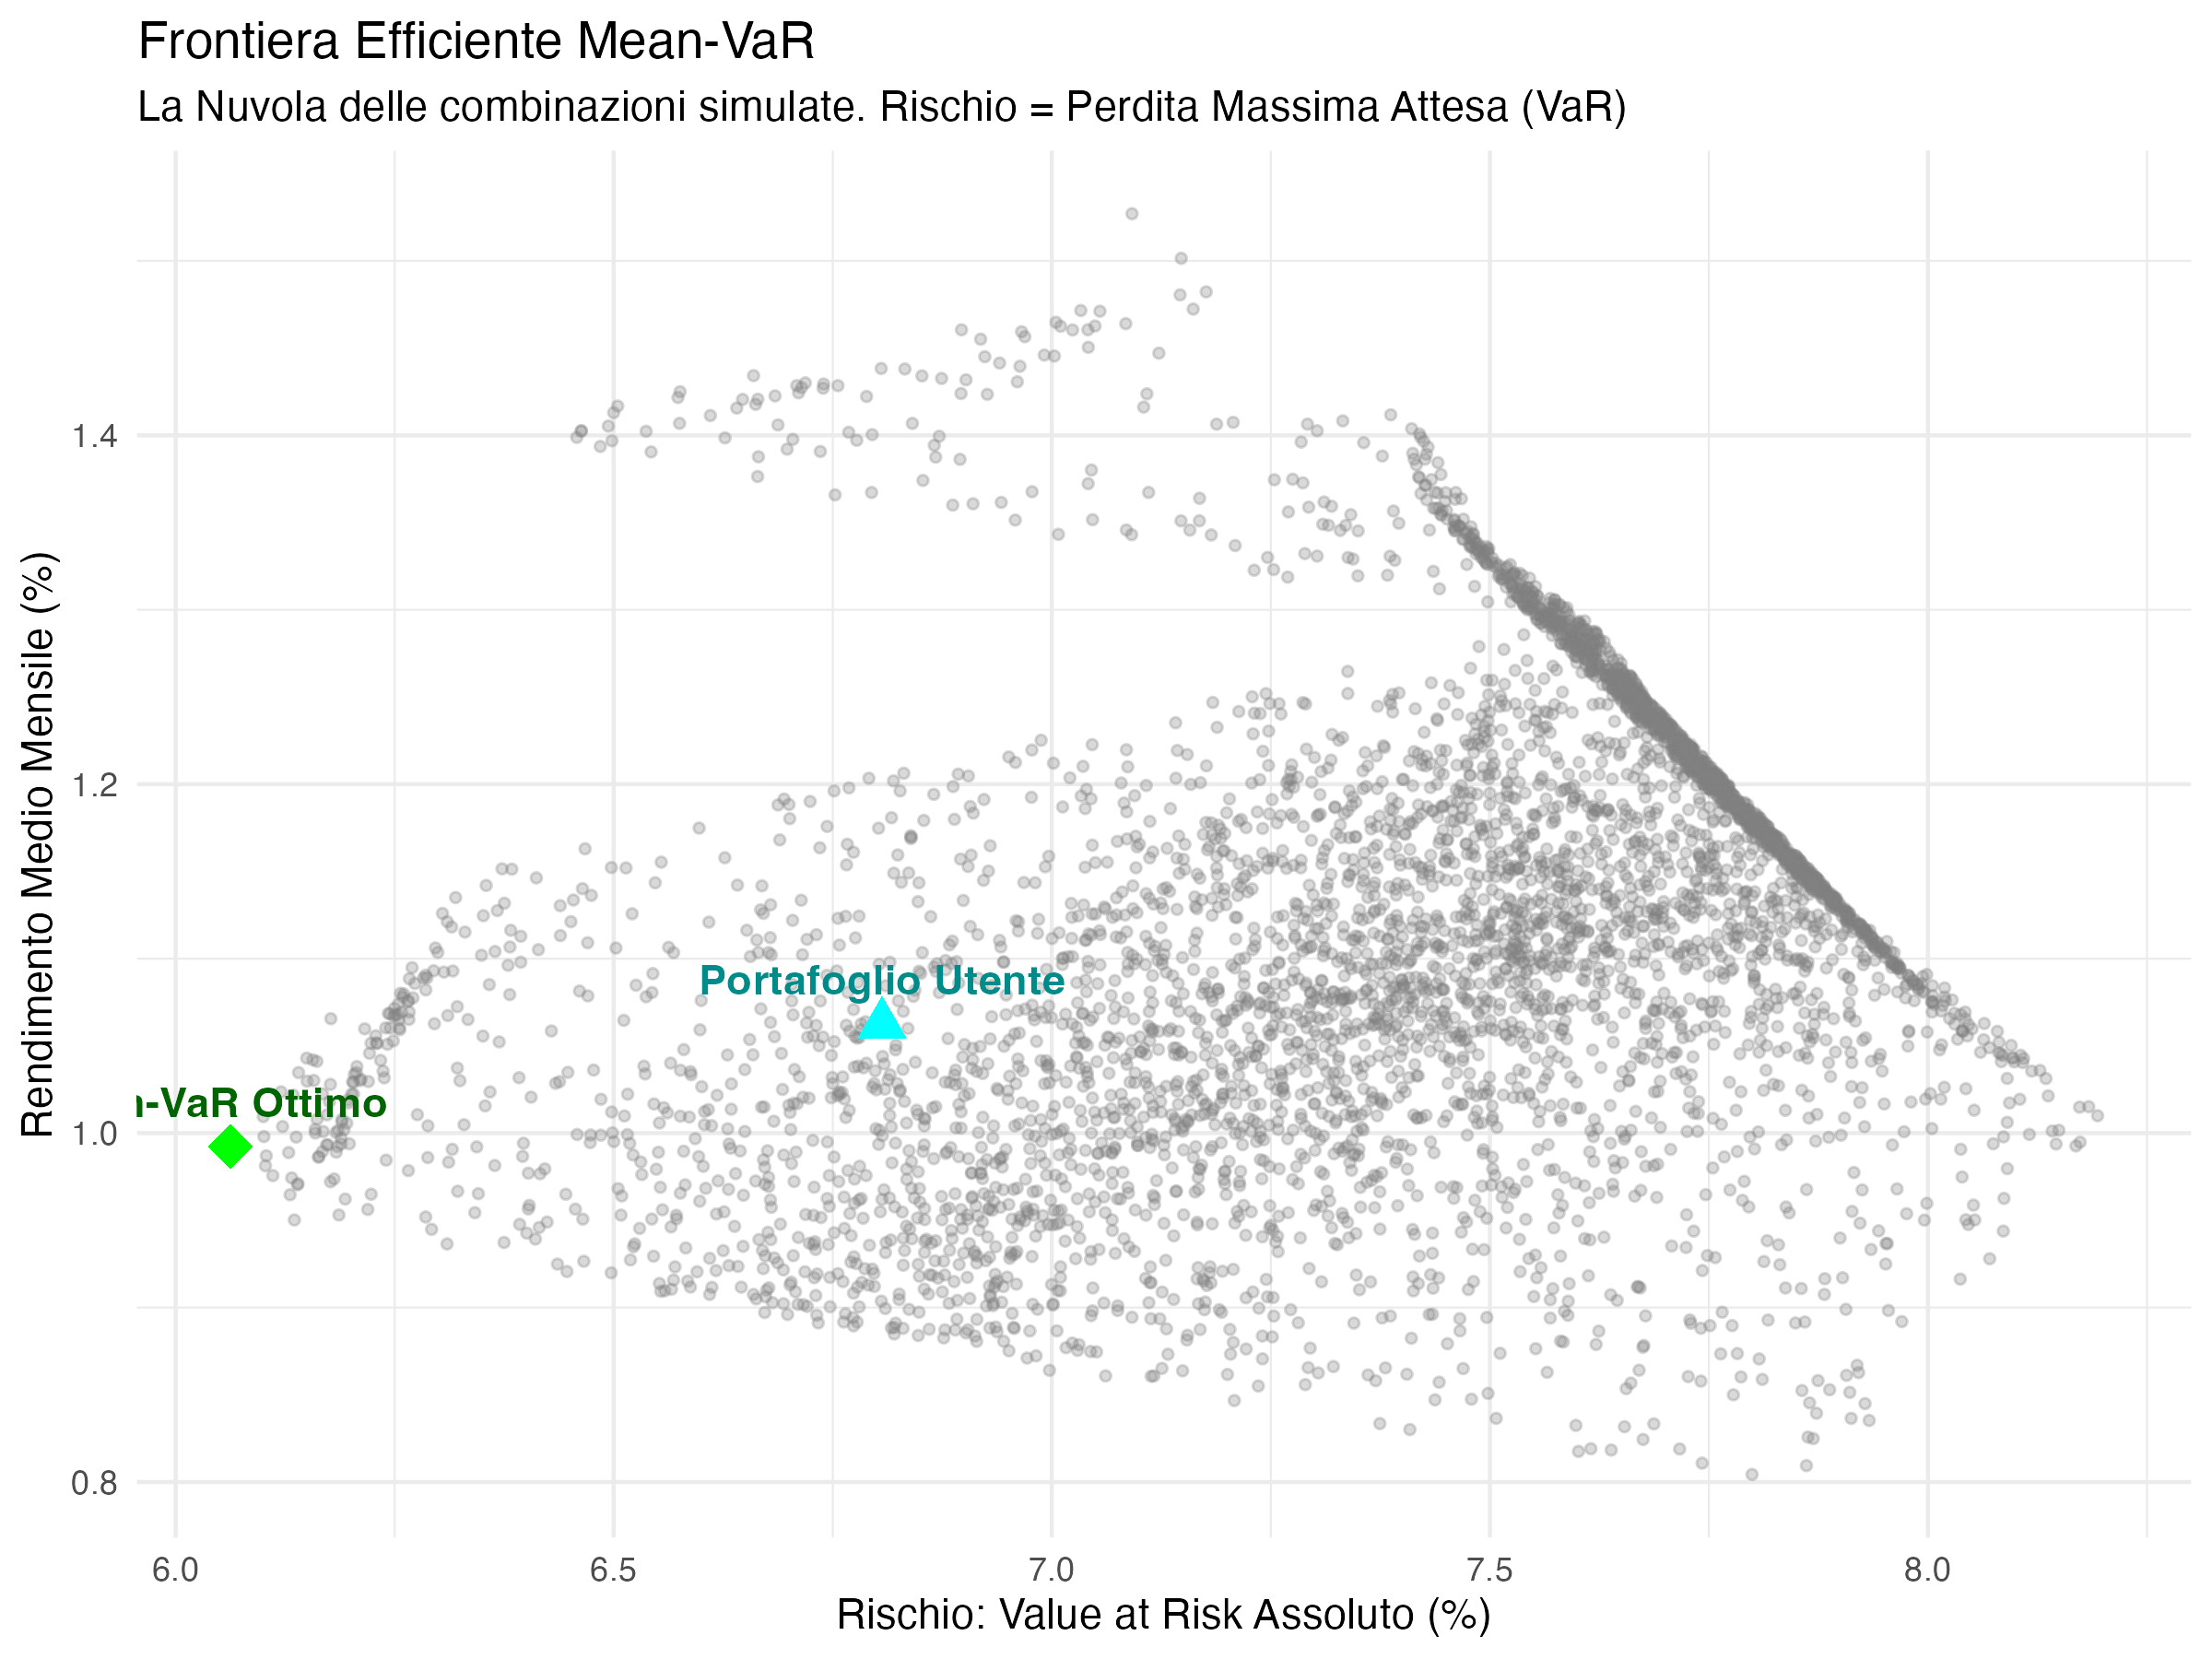
\includegraphics[width=0.9\textwidth]{immagini/markowitz_var_plot.png}
    \caption{Frontiera Efficiente Mean-VaR: Ogni punto rappresenta un'allocazione simulata. Invece della Varianza, sull'asse delle ascisse misuriamo la Perdita Massima Storica attesa al 95\% (VaR). Il diamante verde è il portafoglio a Minimo VaR, mentre il triangolo ciano è un'allocazione equo-pesata dell'utente. Si nota l'evidente "curvatura" di efficienza.}
    \label{fig:min_var_portfolio}
\end{figure}

Il risultato empirico conferma un principio cardine del Risk Management moderno e svela il più grande limite della teoria classica. Mettendo a confronto i due algoritmi sui medesimi dati storici, otteniamo allocazioni diametralmente opposte:
\begin{itemize}
    \item \textbf{Markowitz (Max Sharpe Ratio, Script 8)} alloca circa l'88\% del capitale sul NASDAQ (SXRV) e il 12\% sull'All-World (VWCE). Markowitz osserva che i ritorni medi stellari del settore tecnologico compensano (secondo la metrica della varianza) la sua volatilità, suggerendo un portafoglio aggressivo.
    \item \textbf{Min-VaR (Protezione Fat Tails, Script 10)} ribalta la situazione allocando oltre il 99\% sul VWCE e azzerando il NASDAQ. L'algoritmo non è accecato dai rendimenti medi rialzisti, ma analizza esclusivamente la coda sinistra (il peggior 5\% degli scenari). Nei momenti di crisi (dot-com, 2008, 2022) il NASDAQ subisce crolli (Fat Tails) devastanti, spingendo il Risk Manager matematico a rifugiarsi nell'asset globalmente più diversificato.
\end{itemize}

Quando l'obiettivo matematico primario diviene la protezione dalle catastrofi (Minimizzazione del VaR) piuttosto che la ricerca dell'efficienza Gaussiana, l'algoritmo si sposta verso l'estrema sinistra del grafico, rifiutando gli asset speculativi ad altissimo rendimento/rischio per concentrare il capitale sull'indice più bilanciato.
